%% State of the art (chpt2)
\chapter{State of the art} %8
We begin this work by researching the state of the art in drone hardware, computer vision, and SLAM solutions. All three of these are very active topics with frequent innovations, and we will explore some of them.

\section{Drones}
When talking about autonomous drone navigation, it is important to be aware of what the current hardware is capable of doing, and how we can expect it to evolve in the near future. There is quite a large choice of low-cost drones available to choose from on the market. For civilian UAV's, a tradeoff has to be made between performance (speed, agility, accuracy of sensors, power of embedded computers), battery life, and price. However, it is still a relatively young market, and each year, new drones are created that improve on these quantities.

\subsection{Number of rotors}
Multirotors, or multicopters, are defined as rotorcrafts with three or more rotors. Having more rotors enables them to maneuver in 3D space with fixed-pitch rotors, unlike helicopters, which have articulations at the bases of their rotors. The most common multirotors have 3, 4, 6, or 8 rotors, and are respectively called tricopters, quadcopters (or quadrotors), hexacopters, and octocopters. Having more rotors has the advantage of giving more agility, at the cost of more energy consumption, and therefore a shorter battery life.\\

A free solid object in 3D space, such as a multicopter, has 6 degrees of freedom: 3 for translation and 3 for rotation. To be able to directly control each of these 6 degrees of freedom, it must be possible to give 6 independent controls to the drone. This means that tricopters and quadcopters are always under-actuated: they can't directly control all 6 degrees of freedom.\\

For example, quadrotors whose rotors are all in the same plane (as is almost always the case), can directly control all three of their rotational degrees of freedom, but only one translational degree of freedom, as they can only accelerate in the direction parallel to the rotation of their rotors. Therefore, to control their position in the plane perpendicular to the direction of gravity, they have to first adapt their roll and pitch, so that the resulting force of gravity and the thrust of their rotors points inside that plane. Most hexacopters also work this way, as their rotors are also often in the same plane. Some hexacopters, however, have tilted rotors, and are fully actuated  \cite{dexteroushexrotor}. \\

\begin{figure}[H]
\centering
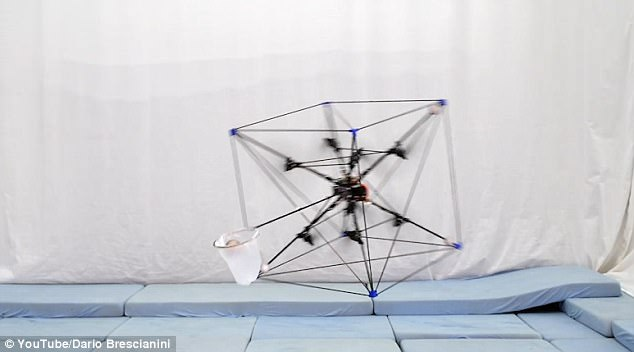
\includegraphics[width=0.6\textwidth]{omnicopter.jpeg}
\caption{The Omnicopter.}
\label{fig:omnicopter}
\end{figure}

Octocopters, on the other hand, are always over-actuated. One example, the Omnicopter, developed at ETH Zurich \cite{omnidirectionalav} can perform a \SI{360}{\degree} rotation along any axis, and move in a straight line in any direction, which enables it to perform complex and precise maneuvers. It is able to catch thrown ping-pong balls with a little net.



\section{Computer Vision}
Computer vision is a very active field of study. Here, we research the state of the art for the two main categories of computer vision tasks we will need to carry out in this thesis: keypoint detection, description and matching, as well as bundle adjustment.

\subsection{Keypoint Detection, Description, and Matching} \label{sec:sota_keypoints}
Keypoint detection will be at the basis of our work, as we will build a map to localize the drone, and this map will be made up of landmarks, visual features observed with the camera of the drone. Good keypoints need to be recognizable from a wide variety of viewpoints, and ideally be invariant to changes of illumination, scale, rotation, or occlusion. Here is a quick overview of some of the most important keypoint detectors and descriptors that exist in the literature.

\subsubsection{Scale-Invariant Feature Transform (SIFT)}
 Published in 1999 by David Lowe from Columbia University, SIFT \cite{sift} is the reference in keypoint description, because it is quite robust. It uses the maxima and minima of a difference of Gaussian function of the image, rescaled at different levels. The image is blurred by Gaussian filters at different scales, and the difference between blurred images is taken. The result is an image without its highest spacial frequencies (noise) and lowest spacial frequencies (untextured parts of the image), leaving only a certain range of frequencies, that correspond to specific detail levels. The maxima and minima of the resulting image are considered to be corners, and become keypoints. Each keypoint is then described by a vector of size \num{128}, representing histograms of orientation in the pixels around the keypoint. SIFT keypoints are very robust to changes of viewpoint, occlusion and illumination. Their main drawback is the computational cost to find them and to extract their descriptor.

\subsubsection{Speeded Up Robust Features (SURF)}
Inspired by SIFT and first published in 2006, Speeded-Up Robust Features \cite{surf} was a new kind of keypoint detector and descriptor. SURF uses square shaped filters to approximate Gaussian smoothing, which can be computed much faster, and then selects points where the determinant of the Hessian matrix is maximal. Its performance in terms of robustness to changes in viewpoint, occlusion, and illumination is similar to that of SIFT but it is computationally much faster.

\subsubsection{Features from Accelerated Segment Test (FAST)}
Published in 2005, the FAST detector \cite{fast} uses a different approach than SIFT and SURF, and is even faster than SURF. FAST compares the intensity of a central pixel with the intensities of the 16 pixels forming a Bresenham circle of radius 3 around the central pixel. If the central pixel is brighter or darker by a certain threshold than N contiguous pixels in the circle, the pixel is considered a corner. This test is very fast, because it is possible to reject points that do not match the criteria without comparing the intensities of all points of the circle. The threshold and the number N are parameters that have to be fixed by the user. In the original version of FAST, $N = 12$ and the four pixels at the cardinal points of the circle (up, down, left, right) are first tested, and the point is rejected if the values of these four points make it impossible for N consecutive brighter or darker pixels to exist.\\

Expanding on this idea, the creators of FAST proposed an upgrade to their algorithm in \cite{fast2} using machine learning. Their upgrade uses the ID3 algorithm to learn a decision tree to decide whether a point is a keypoint or not using the intensities of the 16 pixels. This algorithm automatically selects to best tests to perform on these 16 pixels to quickly decide whether they are corners or not.\\

With this detector, the natural descriptor to use are the intensities of the 16 surrounding pixels, as well as whether the keypoint is a minimum or a maximum. We can already see that the dimension of the descriptor vector of FAST is 16, where SIFT's descriptor is of dimension 128, so we can expect this descriptor to be much less robust than SIFT.
\begin{figure}[H]
\centering
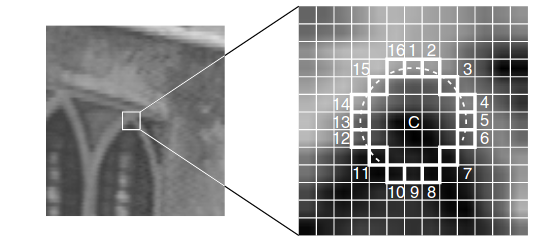
\includegraphics[width=0.6\textwidth]{fast.png}
\caption{Bresenham circle used for FAST. (\cite{fast})}
\label{fig:fast}
\end{figure}

\subsubsection{Binary Robust Independent Elementary Features (BRIEF)}
BRIEF \cite{brief} is a descriptor introduced in 2010 that represents keypoints with binary strings. Each bit in the string is the result of a test testing which one of two specific pixels in the neighborhood of the keypoint is brightest in the smoothed image. Different lengths can be used for the string, but the creators of this descriptor found that a size of only 256 or even 128 bits is often enough for accurate matching. Matching between BRIEF features is done using the Hamming distance, which can be computed very quickly on modern computers.

\subsubsection{Oriented FAST and Rotated BRIEF (ORB)}
In 2011 Rublee et al. \cite{orb} proposed a combination of a modified FAST detector, and a modified BRIEF descriptor, to obtain the ORB detector and descriptor. One of the main drawbacks of FAST is that is has no orientation component, so it is unable to recognize keypoints when these are rotated in the camera plane. ORB computes an orientation component to each keypoint detected by FAST by using the intensity centroid of the patch, and then computes a rotated BRIEF descriptor, so that the resulting keypoint is invariant to rotations. Because the FAST detector and BRIEF descriptor are both very fast methods, and result in very small descriptors, ORB keypoints are very efficient computationally.

\subsection{Bundle Adjustment}
Bundle adjustment is the problem of using a set of images to simultaneously reconstruct a 3D structure and estimate cameras' positions and intrinsic parameters. It was first used in the 1950's in the field of photogrammetry, the science of taking measurements of photographs \cite{bamodernsynthesis}. There exist many open-source libraries solving bundle adjustment problems. SBA (sparse bundle adjustment) \cite{sba} is a library for solving bundle adjustment problems that takes advantage of their sparse structure. Ceres \cite{ceres-solver} is another general-purpose solver that is well suited for solving bundle adjustment problems. Bundler \cite{bundler} is a structure-from-motion system based on SBA that uses bundle adjustment to transform a set of unordered photographs (found on the internet for example) of a common scene to reconstruct it.

\begin{figure}[H]
\centering
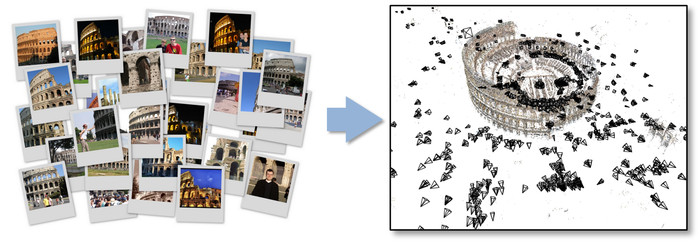
\includegraphics[width=0.6\textwidth]{bundler.jpg}
\caption{Result of bundle adjustment (taken from \cite{bundler})}
\label{fig:bundler}
\end{figure}

\section{Simultaneous Localization And Mapping}
Simultaneous Localization and Mapping (SLAM) refers to the joint task of creating a map of a robot's surroundings, while also keeping track of the robot's location in this map. The word "robot" should be understood very broadly in this context, for example it could be a simple hand-held camera. Because there are countless different types of robots that do SLAM, SLAM is also a very diverse field, with different algorithms for different kinds of sensors.

\subsection{Parallel Tracking and Mapping (PTAM)}
PTAM \cite{ptam} was one of the first applications of Bundle Adjustment in real time. It is able to track the movement of a hand-held camera by constructing a map of visual features (it uses FAST features). It is called parallel tracking and mapping, because the tracking and mapping tasks are completely decoupled, and happen simultaneously in different threads. However, it is quite expensive computationally, so it only works in real time with small workspaces, and lacks loop closure (the ability to correct accumulated errors when revisiting a previously visited location). PTAM has been adapted to work with Parrot AR.Drones at the Technische Universtät München \cite{engel2011msc} with impressive results, however this solutions suffers from PTAM's problems: the size of the map is quite limited, and there is no loop closure. As a result, their implementation builds an initial map, and then stops mapping, only using this initial map for tracking and position control, which makes it unusable as soon as the drone moves away from this initial map.
\newpage
\subsection{ORB-SLAM}
ORB-SLAM \cite{orbslam}, created in 2015 is a keyframe-based monocular visual SLAM that builds a map of ORB features. The creators of ORB-SLAM extended it to ORB-SLAM 2 \cite{orbslam2}, which works with stereo and RGB-D cameras for better accuracy. It uses bundle adjustment to build a consistent map and for loop closure, and works in real time in large environments, by using a covisibility graph to focus the mapping and localization tasks on a small portion of the map at a time. It also uses a survival of the fittest approach to remove redundant keyframes and points.

\subsection{Large-Scale Direct Monocular SLAM (LSD-SLAM)}
Developed at the Technishe Universität München in 2014, LSD-SLAM \cite{lsdslam} uses a semi-dense approach to SLAM. Unlike the previously mentioned methods, it does not use keypoints, but rather, the entire image. Each new image is used to estimate a similarity transform from the previous image to estimate the position of the camera, and is then used to either refine the last keyframe, or create a new one. Each keyframe consists of an image and a depth map created with per-pixel stereo comparisons between consecutive images. The result works in real time on a CPU, and is able to obtain accurate maps of large environments, and to correct accumulated errors after loop closure.

\subsection{Direct Sparse Odometry (DSO)}
Also produced at the TUM, DSO \cite{dso} was created in 2016. Like LSD-SLAM, DSO is a direct method: it works directly on the image pixels by computing an associated depth field, instead of extracting keypoints from the image. Working directly on the image allows to bypass the costly point detection and description steps, and also allows to use points that are not recognizable by themselves, making more data useable (edges, weak intensity regions) and to work in less textured environments. Unlike LSD-SLAM, DSO is a sparse method, it samples a limited number of points on each keyframe, and does not use a smoothness geometry prior. Because DSO permanently marginalizes old points, it cannot detect a loop closure and correct accumulated errors, so it is more a pure visual odometry than a complete SLAM system, and cannot be used to obtain a consistent map (if it visits the same location twice, all points will be doubled). However, it is very accurate, and even after very large loops, the accumulated error remains small. Figure \ref{fig:dsodrift} shows an illustration of the accumulated error of DSO after going through an entire subway station.

\begin{figure}[H]
  \centering
  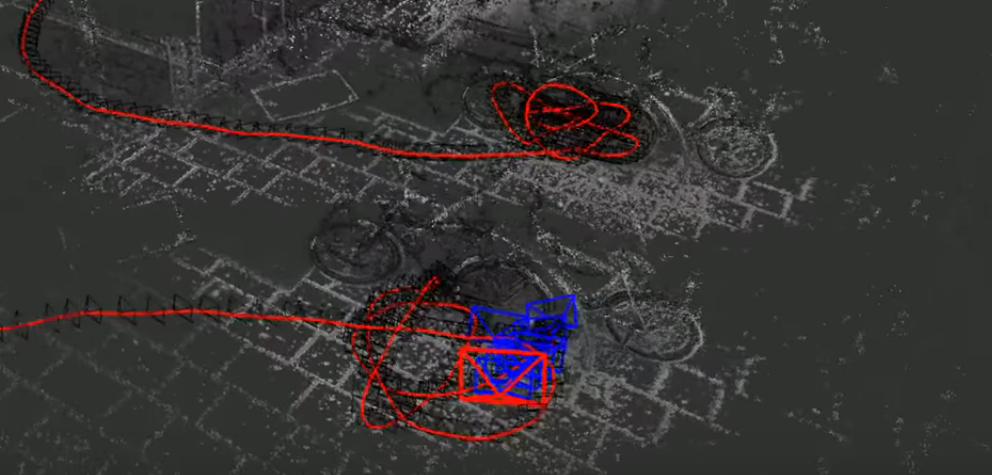
\includegraphics[width=0.75\textwidth]{dsodrift.png}
    \caption{Drift of DSO after going through an entire subway station. We only see the beginning and end of the trajectory (in red). \cite{dsovid}}
    \label{fig:dsodrift}
\end{figure}

\subsection{CNN-SLAM}
CNN-SLAM \cite{cnnslam} uses a deep Convolutional Neural Network (CNN) to learn the depth field from single views of a monocular camera, and then fuses this information with depth measurements obtained from a keyframe-based monocular SLAM. It also incorporates a second CNN to learn semantic labels from a single view, to learn what parts of the scene constitutes floors, walls, or other objects. Their use of a CNN allows to overcome one of monocular SLAM's main challenges: scale estimation, because it gives an absolute estimation of the scale at every frame, preventing the scale from drifting over time.

\begin{figure}[H]
  \centering
  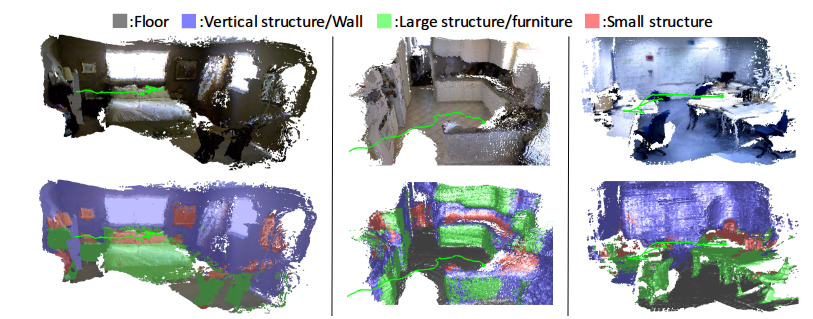
\includegraphics[width=0.75\textwidth]{cnnslam.png}
    \caption{Result of CNN-SLAM, with semantic labels. \cite{cnnslam}}
    \label{fig:cnnslam}
\end{figure}
